% Provenance (never printed): cycle 2 "Questionner le monde" (states of water in
% weather phenomena; daily observation), see sources/book1/PROVENANCE.md.
% Book 1, grade 1, chapter 1. No real-world number in this chapter.
\chapter{Observar el tiempo}\label{ch:g1:watching-the-weather}

Es muy temprano. Lena se despierta, se sube a la silla que hay junto a la
ventana de su cuarto y mira fuera. El cielo está gris. Unas gotitas de agua
resbalan por el cristal. Los tejados de enfrente están mojados y brillan, y
el árbol del jardín gotea.

---¿Qué me pongo hoy? ---se pregunta.

Para responder, Lena no necesita ningún libro ni ninguna máquina. Le basta
con mirar por la ventana. La ventana es su primera estación meteorológica.

\begin{omfigure}
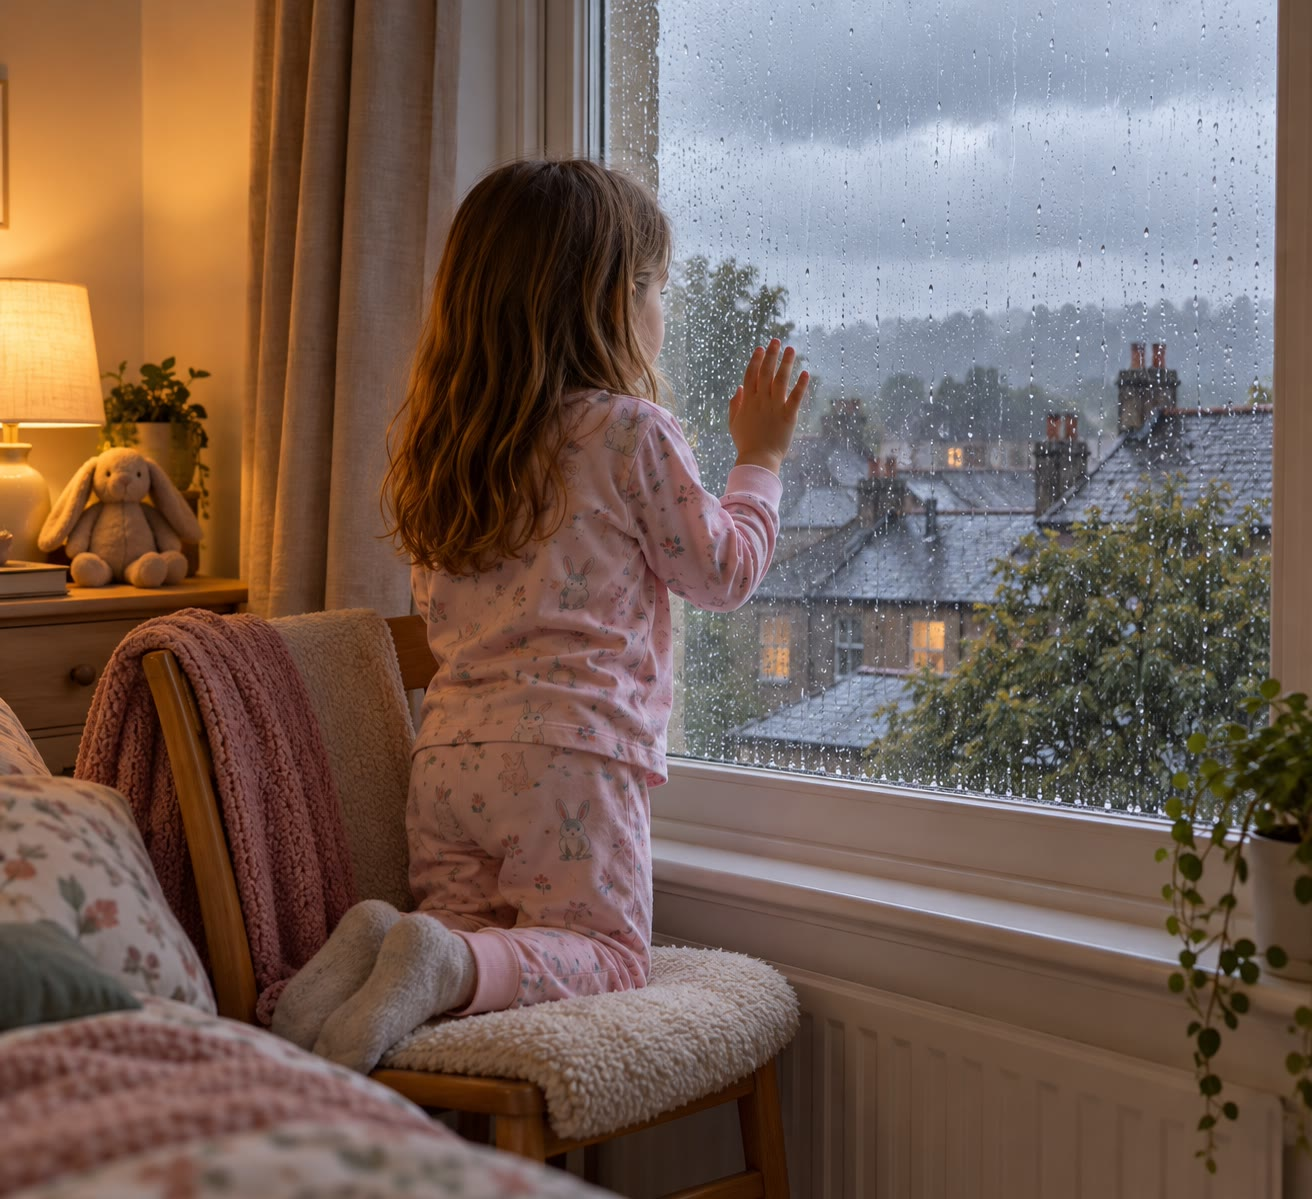
\includegraphics[width=0.72\linewidth]{images/book1/ai/g1-rainy-window.jpg}

{\small Una mañana gris y lluviosa vista a través de una ventana.}
\end{omfigure}

\begin{recall}
Cada mañana sale el Sol y empieza el día; cada tarde se pone y llega la
noche. En los libros de física has visto por qué la noche sigue al día. En
este capítulo miramos otra cosa que cambia todo el tiempo: el \omterm{def:g1:watching-the-weather:weather}{tiempo} que
hace.
\end{recall}

\section{¿Qué es el tiempo?}

Cuando salimos a la calle, notamos el aire en la cara. Puede ser cálido o
frío. Puede estar quieto, o puede empujarnos el pelo y la ropa: entonces
hace viento. Miramos al cielo. Puede estar azul y luminoso, o cubierto de
nubes. A veces cae lluvia de las nubes, a veces nieve. Todo esto junto es
el \omterm{def:g1:watching-the-weather:weather}{tiempo}.

\begin{definition}[El tiempo]\label{def:g1:watching-the-weather:weather}
El \emph{tiempo}\index{tiempo} es cómo están el aire y el cielo en un lugar
y en un momento: soleado o nublado, seco, lluvioso o con nieve, en calma o
con viento, cálido o frío.
\end{definition}

Para describir el \omterm{def:g1:watching-the-weather:weather}{tiempo}, respondemos a unas pocas preguntas sencillas:
\begin{enumerate}
  \item \textbf{¿Cómo está el cielo?} ¿Está azul, con el Sol brillando?
        ¿Hay unas pocas nubes, o está todo gris?
  \item \textbf{¿Cae algo del cielo?} ¿Lluvia? ¿Nieve? ¿Nada?
  \item \textbf{¿Hace viento?} ¿Se mueven las hojas de los árboles? ¿Ondea
        una bandera?
  \item \textbf{¿Hace calor o frío?} ¿Necesitamos abrigo?
\end{enumerate}

\begin{omfigure}
\begin{minipage}[b]{0.49\linewidth}\centering
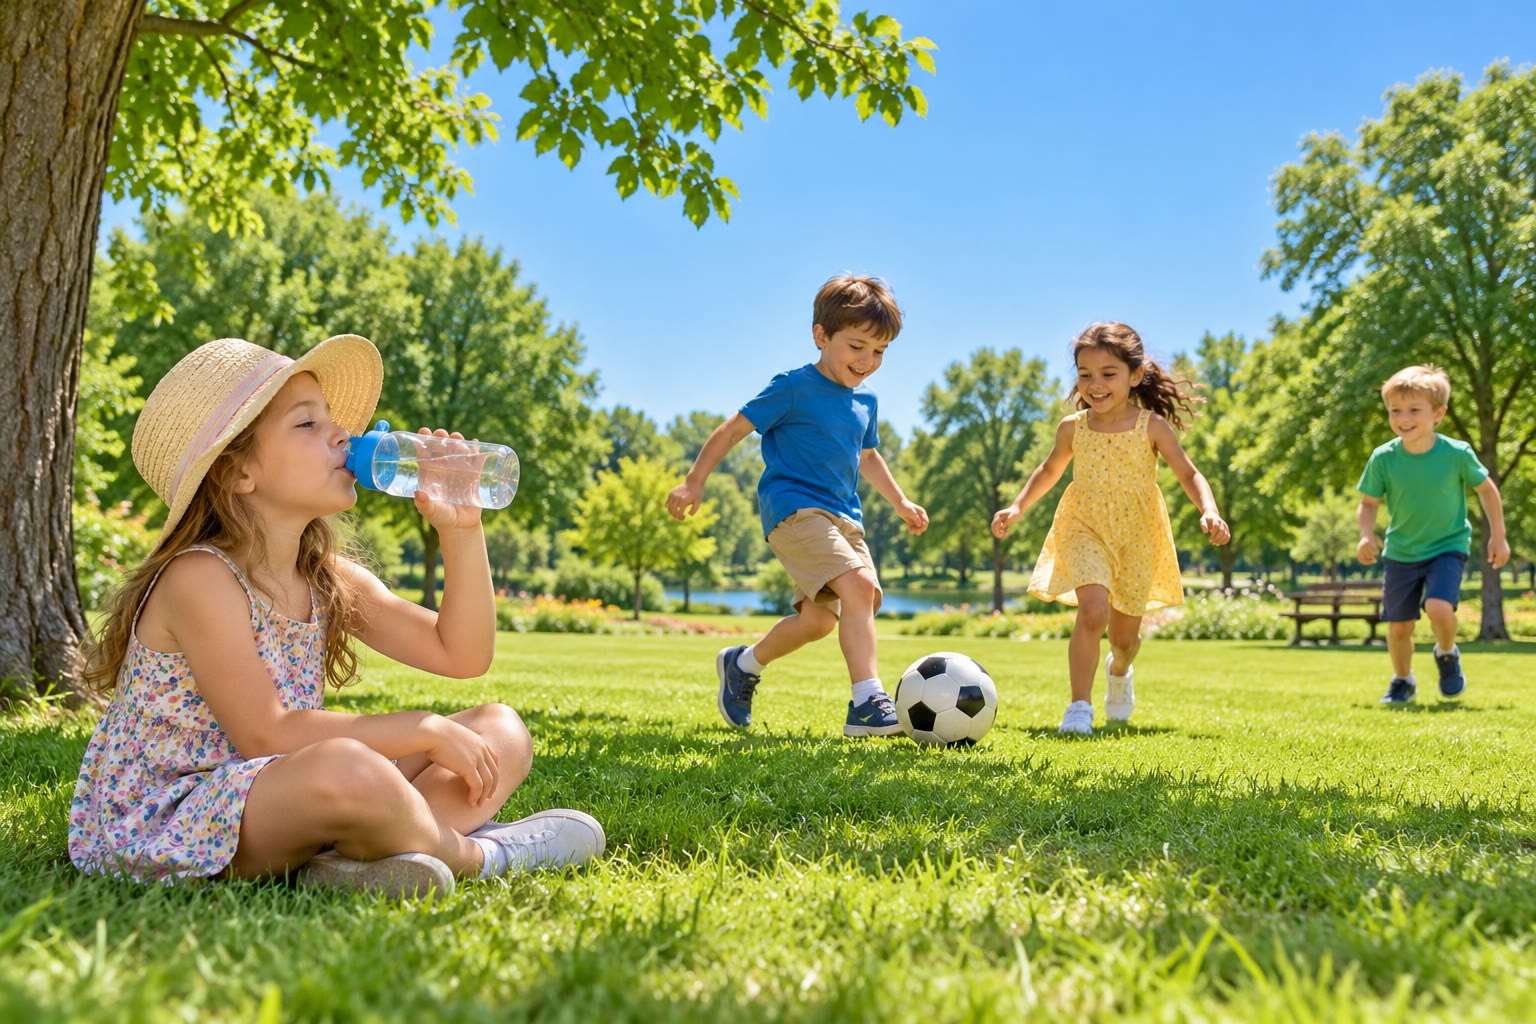
\includegraphics[width=\linewidth]{images/book1/ai/g1-sunny-park.jpg}

{\small Sol y calor.}
\end{minipage}\hfill
\begin{minipage}[b]{0.49\linewidth}\centering
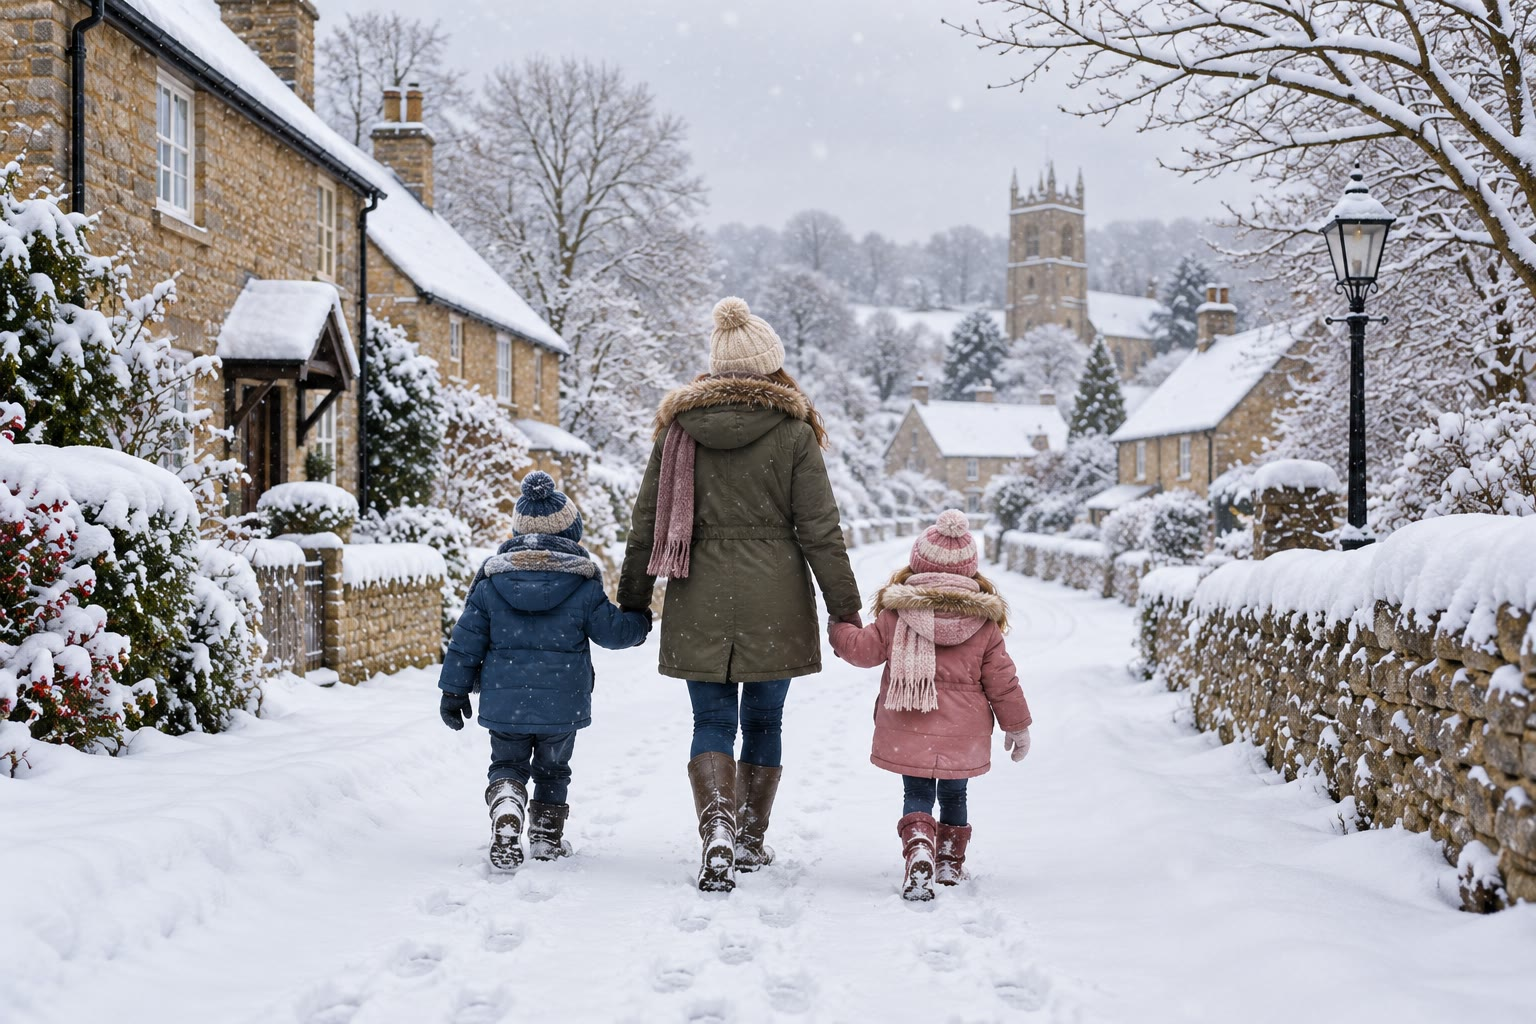
\includegraphics[width=\linewidth]{images/book1/ai/g1-snowy-street.jpg}

{\small Nieve y frío.}
\end{minipage}

\medskip
\begin{minipage}[b]{0.49\linewidth}\centering
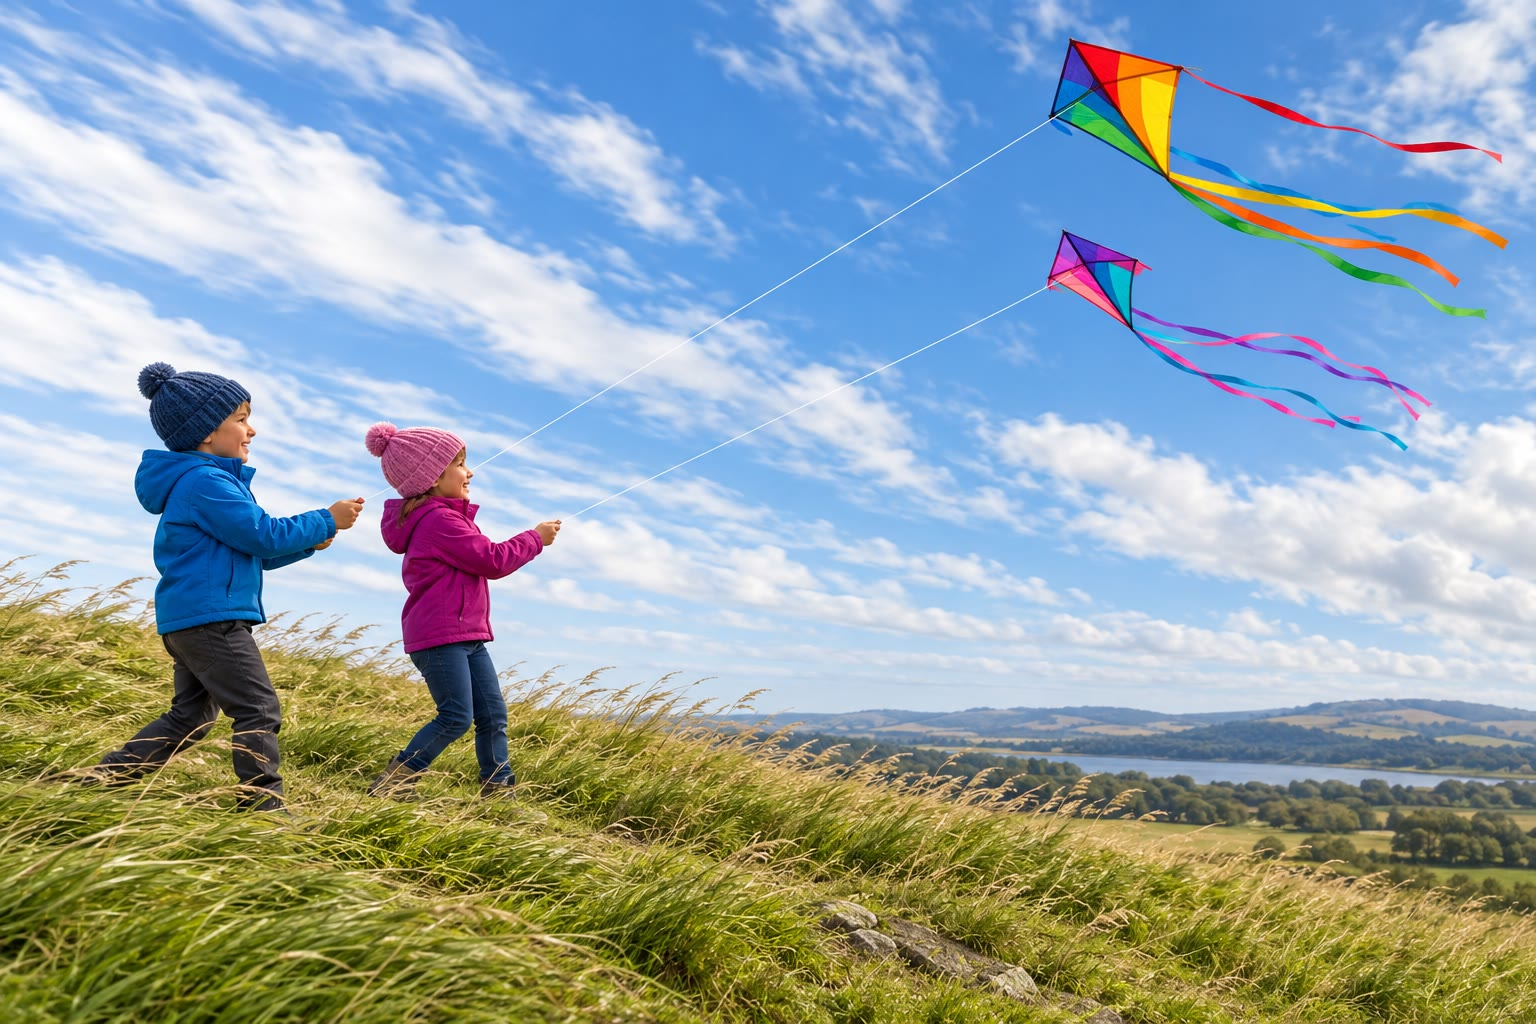
\includegraphics[width=\linewidth]{images/book1/ai/g1-windy-kites.jpg}

{\small Viento: las cometas vuelan.}
\end{minipage}\hfill
\begin{minipage}[b]{0.49\linewidth}\centering
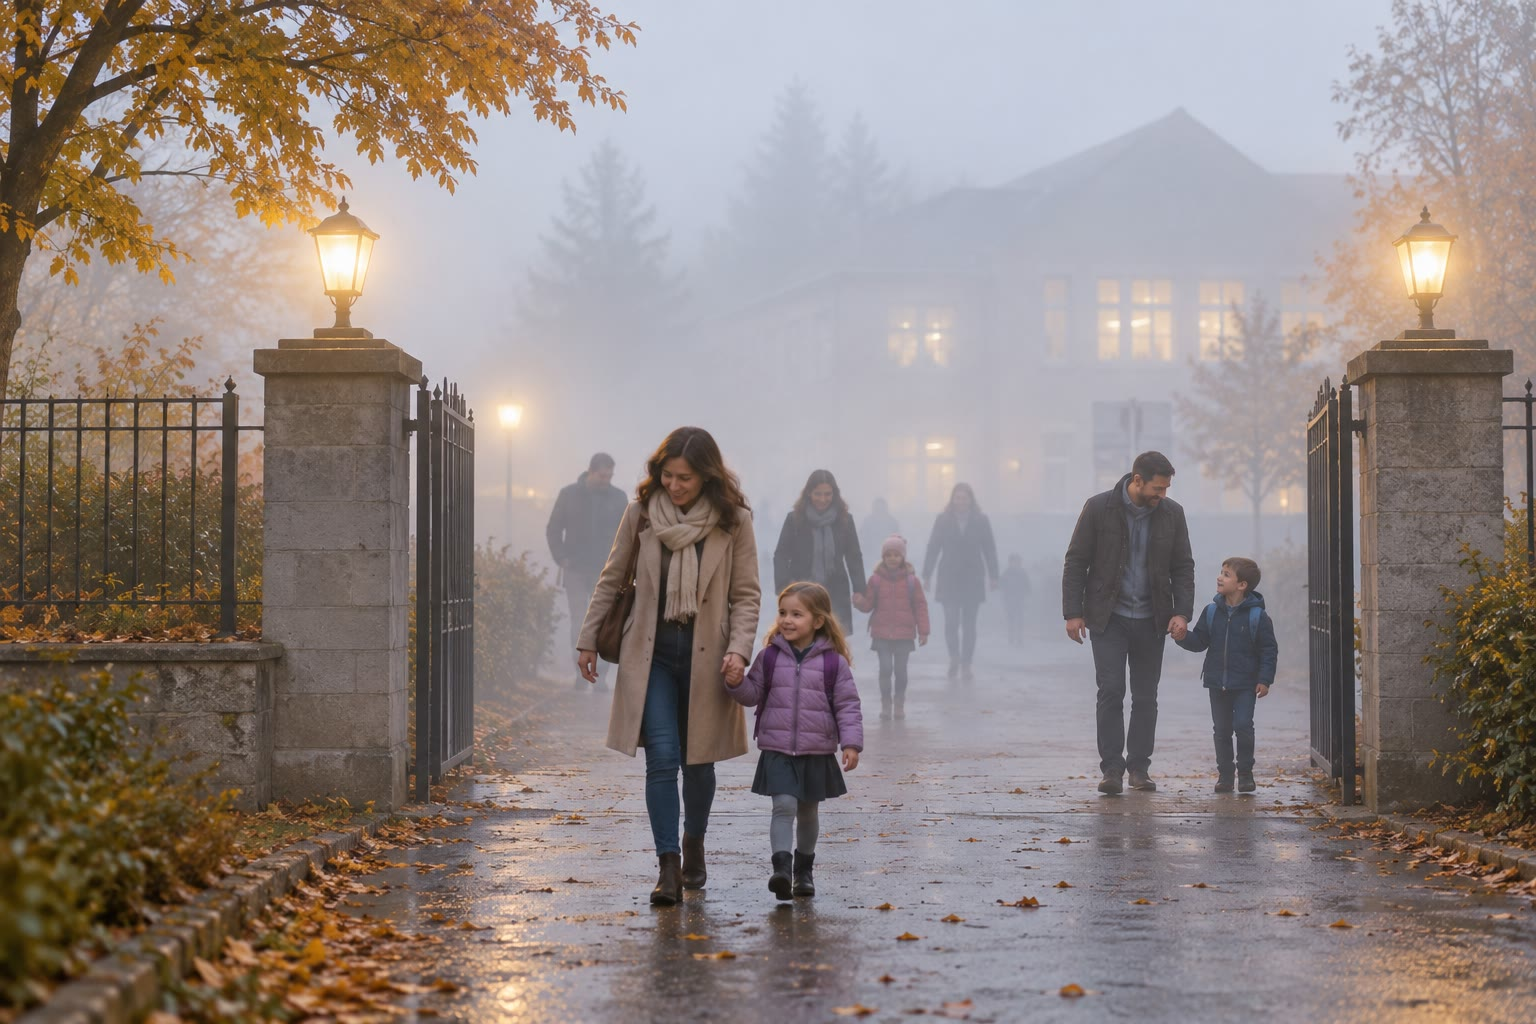
\includegraphics[width=\linewidth]{images/book1/ai/g1-foggy-school.jpg}

{\small Niebla: no se ve lejos.}
\end{minipage}
\end{omfigure}

\begin{example}[La niebla]\label{ex:g1:watching-the-weather:fog}
Algunas mañanas el propio aire parece blanco, y los árboles del final de la
calle parecen desaparecer. Es la niebla. La niebla es una nube que toca el
suelo. Cuando el día se calienta, la niebla suele desaparecer.
\end{example}

\section{Los símbolos del tiempo y la tabla del tiempo}

Describir el \omterm{def:g1:watching-the-weather:weather}{tiempo} con palabras lleva mucho rato. Quienes observan el
\omterm{def:g1:watching-the-weather:weather}{tiempo} usan en su lugar unos dibujitos: los \omterm{def:g1:watching-the-weather:weather-chart}{símbolos del tiempo}. Cada
símbolo es fácil de dibujar y fácil de reconocer.

\begin{omfigure}
\begin{tikzpicture}[x=1cm, y=1cm]
  \foreach \i/\n/\t in {0/sun/soleado, 1/suncloud/sol y nubes,
      2/cloud/nublado, 3/rain/lluvioso, 4/shower/chubascos} {
    \pic[scale=1.25, transform shape] at (\i*2.6,0) {omwx=\n};
    \node[font=\small, align=center, text width=2.4cm] at (\i*2.6,-1.05) {\t};
  }
  \foreach \i/\n/\t in {0/snow/nieve, 1/storm/tormenta, 2/fog/niebla,
      3/wind/viento} {
    \pic[scale=1.25, transform shape] at (\i*2.6+1.3,-2.6) {omwx=\n};
    \node[font=\small, align=center, text width=2.4cm] at (\i*2.6+1.3,-3.65) {\t};
  }
\end{tikzpicture}

{\small Nueve \omterm{def:g1:watching-the-weather:weather-chart}{símbolos del tiempo}. La tormenta tiene una nube oscura y un
rayo; los chubascos llegan con ratos de sol entre ellos.}
\end{omfigure}

\begin{definition}[Tabla del tiempo]\label{def:g1:watching-the-weather:weather-chart}
Un \emph{símbolo del tiempo}\index{simbolo del tiempo@símbolo del tiempo} es
un dibujo pequeño que muestra una clase de \omterm{def:g1:watching-the-weather:weather}{tiempo}. Una \emph{tabla del
tiempo}\index{tabla del tiempo} es un cuadro en el que anotamos, día tras
día, el \omterm{def:g1:watching-the-weather:weather}{tiempo} que hemos visto, con símbolos del \omterm{def:g1:watching-the-weather:weather}{tiempo}.
\end{definition}

Una clase puede llevar una \omterm{def:g1:watching-the-weather:weather-chart}{tabla del tiempo} durante toda una semana. Cada
mañana, y otra vez cada tarde, un niño o una niña mira fuera y dibuja el
símbolo en la casilla correcta. También anotamos si hace calor o frío.

\begin{omfigure}
\begin{tikzpicture}[x=1cm, y=1cm]
  \def\cw{1.9}
  \foreach \d [count=\i from 0] in {Lunes, Martes, Miércoles, Jueves,
      Viernes, Sábado, Domingo}
    \node[font=\scriptsize\bfseries] at ({1.6+\i*\cw+\cw/2},0.35) {\d};
  \node[font=\scriptsize\bfseries, anchor=east] at (1.45,-0.5) {mañana};
  \node[font=\scriptsize\bfseries, anchor=east] at (1.45,-1.5) {tarde};
  \node[font=\scriptsize\bfseries, anchor=east, align=right] at (1.45,-2.35) {¿calor\\o frío?};
  \draw[black!60] (1.6,0) rectangle ({1.6+7*\cw},-2.7);
  \foreach \i in {1,...,6}
    \draw[black!60] ({1.6+\i*\cw},0.65) -- ({1.6+\i*\cw},-2.7);
  \draw[black!60] (1.6,0.65) -- ({1.6+7*\cw},0.65);
  \draw[black!60] (1.6,0.65) -- (1.6,0);
  \draw[black!60] ({1.6+7*\cw},0.65) -- ({1.6+7*\cw},0);
  \draw[black!60] (1.6,-1) -- ({1.6+7*\cw},-1);
  \draw[black!60] (1.6,-2) -- ({1.6+7*\cw},-2);
  \foreach \i/\m/\a/\w in {0/rain/rain/frío, 1/cloud/suncloud/frío,
      2/sun/sun/calor, 3/sun/suncloud/calor, 4/suncloud/shower/calor,
      5/fog/sun/calor, 6/cloud/rain/frío} {
    \pic[scale=0.8, transform shape] at ({1.6+\i*\cw+\cw/2},-0.5) {omwx=\m};
    \pic[scale=0.8, transform shape] at ({1.6+\i*\cw+\cw/2},-1.5) {omwx=\a};
    \node[font=\scriptsize] at ({1.6+\i*\cw+\cw/2},-2.35) {\w};
  }
\end{tikzpicture}

{\small La \omterm{def:g1:watching-the-weather:weather-chart}{tabla del tiempo} de una clase durante una semana de primavera.}
\label{fig:g1:watching-the-weather:chart}
\end{omfigure}

\begin{method}[Leer una tabla del tiempo]\label{met:g1:watching-the-weather:read}
Para leer una \omterm{def:g1:watching-the-weather:weather-chart}{tabla del tiempo}:
\begin{enumerate}
  \item busca la columna del día que quieres;
  \item mira la fila: la de la mañana o la de la tarde;
  \item di qué \omterm{def:g1:watching-the-weather:weather}{tiempo} muestra el símbolo.
\end{enumerate}
Para saber cuántos días hizo sol, recorre una fila con el dedo y cuenta los
símbolos del sol.
\end{method}

\begin{example}[Leer la tabla de la clase]\label{ex:g1:watching-the-weather:read}
En la tabla de esta clase, el lunes por la mañana llovió e hizo frío. El
miércoles hizo sol todo el día. El sábado, la niebla de la mañana dejó paso
al sol por la tarde. En las mañanas de la semana, la clase dibujó el sol
2 días: el miércoles y el jueves.
\end{example}

\section{El tiempo cambia}

El \omterm{def:g1:watching-the-weather:weather}{tiempo} no se queda siempre igual. Cambia a lo largo del día, de un día
para otro y a lo largo del año.

\begin{itemize}
  \item \textbf{A lo largo de un día.} Una mañana gris puede convertirse en
        una tarde soleada. Una mañana azul y despejada puede terminar en
        tormenta. Al amanecer y por la noche suele hacer más fresco que por
        la tarde.
  \item \textbf{De un día para otro.} Mira la tabla de la clase: no hay dos
        días de la semana exactamente iguales.
  \item \textbf{A lo largo del año.} En verano los días suelen ser
        cálidos, y en invierno suelen ser fríos; en muchos lugares solo
        nieva en invierno. Los libros de física explican por qué las
        estaciones vuelven cada año.
\end{itemize}

\begin{omfigure}
\begin{tikzpicture}[x=1cm, y=1cm]
  \draw[black!50, line width=0.8pt, -{Stealth[length=2.5mm]}] (0,0) -- (12.2,0);
  \foreach \x/\n/\t/\h in {0.9/fog/primera hora/fresco, 3.5/suncloud/mañana/templado,
      6.1/sun/tarde/calor, 8.7/storm/final de la tarde/calor y tormenta,
      11.2/suncloud/anochecer/más fresco} {
    \pic[scale=1.1, transform shape] at (\x,0.85) {omwx=\n};
    \fill[black!60] (\x,0) circle (1.5pt);
    \node[font=\scriptsize\bfseries, below] at (\x,-0.12) {\t};
    \node[font=\scriptsize, below] at (\x,-0.5) {\h};
  }
\end{tikzpicture}

{\small Un día de verano, de la mañana a la noche: el \omterm{def:g1:watching-the-weather:weather}{tiempo} cambia cinco
veces.}
\label{fig:g1:watching-the-weather:day}
\end{omfigure}

\begin{omfigure}
\begin{tikzpicture}[x=1cm, y=1cm]
  \foreach \i/\s/\c/\g/\w/\gr in {0/primavera/green!55!black/pink!60/suncloud/green!35,
      1/verano/green!45!black/green!50!black/sun/green!35,
      2/otoño/orange!80!black/orange!70/rain/green!25!brown!30,
      3/invierno/black!55/white/snow/white} {
    \begin{scope}[shift={(\i*3.15,0)}]
      \draw[black!30, rounded corners=3pt, fill=ocBlue!6] (-1.4,-0.45) rectangle (1.4,3.05);
      \fill[\gr] (-1.4,-0.45) rectangle (1.4,0);
      \draw[black!25] (-1.4,0) -- (1.4,0);
      \fill[brown!60!black] (-0.09,0) rectangle (0.09,1.0);
      \draw[brown!60!black, line width=1.6pt] (0,0.75) -- (-0.5,1.35);
      \draw[brown!60!black, line width=1.6pt] (0,0.9) -- (0.45,1.45);
      \ifnum\i<3
        \fill[\c, opacity=0.85] (0,1.55) circle (0.72);
        \ifnum\i=0 \foreach \a in {20,80,140,200,260,320} \fill[\g] (0,1.55) ++(\a:0.45) circle (0.09); \fi
        \ifnum\i=2 \foreach \x/\y in {-0.9/0.15,0.7/0.3,0.95/0.1} \fill[\g] (\x,\y) circle (0.07); \fi
      \else
        \draw[white, line width=2.4pt] (-0.5,1.35) -- (-0.35,1.17);
        \draw[white, line width=2.4pt] (0.45,1.45) -- (0.3,1.27);
      \fi
      \pic[scale=0.8, transform shape] at (0.95,2.55) {omwx=\w};
      \node[font=\small\bfseries] at (0,-0.75) {\s};
    \end{scope}
  }
\end{tikzpicture}

{\small El mismo árbol en las cuatro estaciones: flores en primavera, hojas
verdes y espesas en verano, hojas anaranjadas que caen en otoño, ramas
desnudas con nieve en invierno.}
\label{fig:g1:watching-the-weather:seasons}
\end{omfigure}

\begin{remark}[¿De dónde viene el viento?]\label{rem:g1:watching-the-weather:wind}
El viento no se ve, pero sí vemos lo que hace. Una bandera, una manga de
viento o el humo de una chimenea son empujados por el viento: señalan hacia
donde va el viento, así que el viento viene del otro lado.
\end{remark}

\begin{omfigure}
\begin{tikzpicture}[x=1cm, y=1cm]
  % ground
  \fill[green!30!omLithAlluv] (-0.4,-0.1) rectangle (8.4,0);
  % windsock on a pole
  \draw[black!70, line width=1.2pt] (1,0) -- (1,3.2);
  \fill[orange!85, draw=black!60] (1,3.15) -- (3.4,2.95) -- (3.4,2.55) -- (1,2.45) -- cycle;
  \fill[white] (1.6,3.1) -- (2.2,3.05) -- (2.2,2.5) -- (1.6,2.47) -- cycle;
  \fill[white] (2.8,3.0) -- (3.4,2.95) -- (3.4,2.55) -- (2.8,2.53) -- cycle;
  \draw[black!60] (1,3.15) -- (3.4,2.95) -- (3.4,2.55) -- (1,2.45);
  % flag
  \draw[black!70, line width=1.2pt] (5.4,0) -- (5.4,3.2);
  \fill[ocBlue!70, draw=black!60] (5.4,3.15) .. controls (6.0,3.3) and (6.4,2.9) .. (7.1,3.05)
     -- (7.1,2.35) .. controls (6.4,2.2) and (6.0,2.6) .. (5.4,2.45) -- cycle;
  % wind arrows
  \foreach \y in {1.0,1.6}
    \draw[omWxRain, line width=1.4pt, -{Stealth[length=3mm]}] (-0.3,\y) -- (0.7,\y);
  \node[font=\small, align=right, anchor=east] at (-0.45,1.3) {el viento\\viene de aquí};
  \draw[black!60, -{Stealth[length=2mm]}] (4.1,2.75) -- (4.9,2.75);
  \node[font=\small, align=left, anchor=west] at (7.5,2.7) {la bandera y la\\manga señalan\\adónde va el viento};
\end{tikzpicture}

{\small Una manga de viento y una bandera en un día de viento. El viento
sopla de izquierda a derecha.}
\end{omfigure}

\section{¿Para qué observamos el tiempo?}

Mucha gente necesita saber qué \omterm{def:g1:watching-the-weather:weather}{tiempo} va a hacer.
\begin{itemize}
  \item \textbf{Los agricultores} miran el cielo antes de segar el heno: la
        lluvia lo echaría a perder. En primavera temen una noche de helada
        que podría matar las plantas jóvenes.
  \item \textbf{Los marineros y los pescadores} vigilan el viento: un viento
        fuerte levanta olas grandes, y los barcos se quedan en el puerto.
  \item \textbf{Los pilotos} necesitan saber si hay niebla, tormentas o
        viento antes de que despegue un avión.
  \item \textbf{Una clase} que va de excursión al bosque quiere saber si
        debe llevar impermeables o gorras para el sol.
\end{itemize}
Cada día, unas personas llamadas meteorólogos observan el \omterm{def:g1:watching-the-weather:weather}{tiempo} en todo el
mundo y nos cuentan, por la radio, la televisión o el teléfono, qué \omterm{def:g1:watching-the-weather:weather}{tiempo}
hará probablemente en los próximos días.

\begin{example}[Señales en el cielo]\label{ex:g1:watching-the-weather:signs}
Mucho antes de que existieran la radio y los teléfonos, la gente aprendió a
leer el cielo. Cuando unas nubecillas blancas crecen, por la tarde, hasta
formar altas torres oscuras, se acerca un chubasco o una tormenta. Cuando el
viento cambia y el cielo se va cubriendo poco a poco de un velo gris, la
lluvia suele llegar unas horas después. Estas señales no siempre aciertan,
pero a menudo son útiles.
\end{example}

\section{Vestirse según el tiempo}

Ahora Lena ya puede responder a su pregunta. Llueve y hace frío, así que se
pondrá el impermeable y las botas. Mañana el \omterm{def:g1:watching-the-weather:weather}{tiempo} puede ser distinto, y
volverá a elegir.

\begin{omfigure}
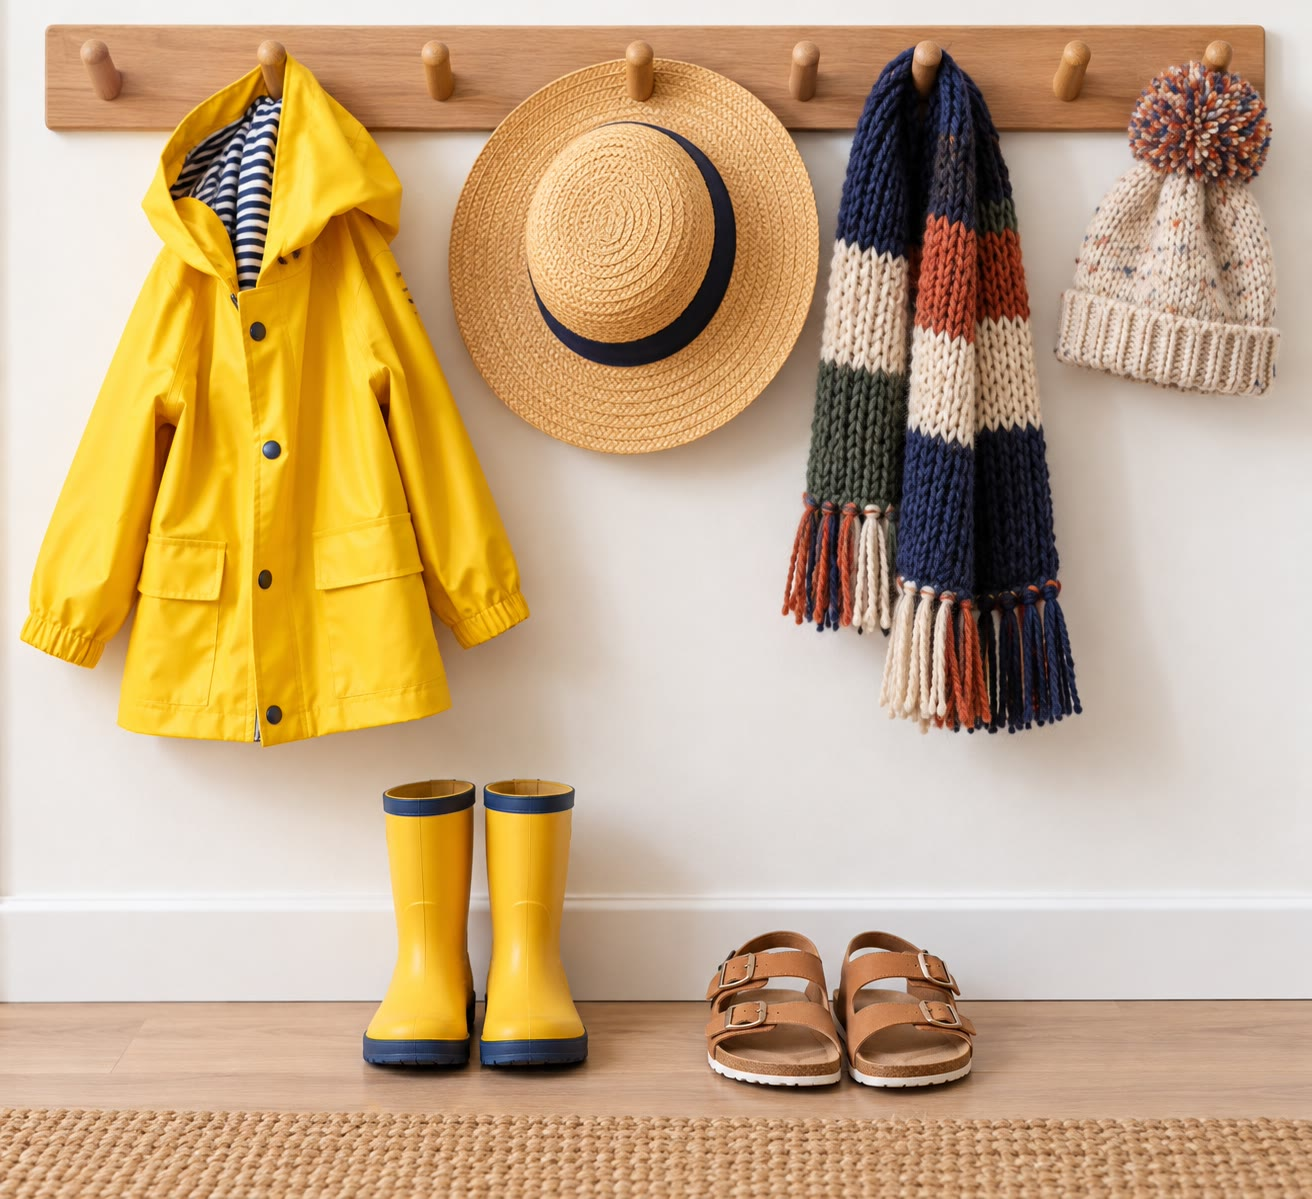
\includegraphics[width=0.66\linewidth]{images/book1/ai/g1-coat-pegs.jpg}

{\small Ropa para cada clase de \omterm{def:g1:watching-the-weather:weather}{tiempo}: un impermeable, una gorra para el
sol, una bufanda y un gorro de lana, unas botas y unas sandalias.}
\end{omfigure}

\begin{method}[Elegir la ropa según el tiempo]\label{met:g1:watching-the-weather:clothes}
Mira el cielo y nota el aire; después:
\begin{itemize}
  \item lluvia o chubascos: un impermeable o un paraguas, y botas;
  \item frío o nieve: un abrigo caliente, una bufanda, un gorro y guantes;
  \item sol fuerte y calor: una gorra, ropa ligera y agua para beber;
  \item viento: un abrigo que cierre bien; el paraguas no sirve de mucho.
\end{itemize}
\end{method}

\begin{safety}
\textbf{No mires nunca directamente al Sol}, ni siquiera un momento, y
nunca a través de unas gafas, unos prismáticos o una cámara: puede dañarte
los ojos para siempre. Cuando hay tormenta, quédate dentro de casa o en un
coche, aléjate de los árboles altos y del agua, y espera a que pase la
tormenta.
\end{safety}

\section{Ejercicios}

\begin{exercise}[$\star$]\label{exo:g1:watching-the-weather:1}
Dibuja el símbolo de cada clase de \omterm{def:g1:watching-the-weather:weather}{tiempo}: soleado; lluvioso; con nieve;
nublado.
\end{exercise}

\begin{exercise}[$\star$]\label{exo:g1:watching-the-weather:2}
¿Qué \omterm{def:g1:watching-the-weather:weather}{tiempo} hace en cada una de las cuatro fotos de la sección
``¿Qué es el \omterm{def:g1:watching-the-weather:weather}{tiempo}?''? Usa una o dos palabras para cada una.
\end{exercise}

\begin{exercise}[$\star$]\label{exo:g1:watching-the-weather:3}
Mira la \omterm{def:g1:watching-the-weather:weather-chart}{tabla del tiempo} de la clase. ¿Qué \omterm{def:g1:watching-the-weather:weather}{tiempo} hizo el martes por la
mañana? ¿Y el viernes por la tarde? ¿Y el domingo por la tarde?
\end{exercise}

\begin{exercise}[$\star$]\label{exo:g1:watching-the-weather:4}
En la \omterm{def:g1:watching-the-weather:weather-chart}{tabla del tiempo} de la clase, ¿qué día hizo sol por la mañana y por
la tarde?
\end{exercise}

\begin{exercise}[$\star$]\label{exo:g1:watching-the-weather:5}
Une cada prenda con un tiempo: una gorra para el sol; unas botas y un
impermeable; una bufanda y unos guantes. Los \omterm{def:g1:watching-the-weather:weather}{tiempos} son: frío y con nieve;
calor y sol; lluvioso.
\end{exercise}

\begin{exercise}[$\star$]\label{exo:g1:watching-the-weather:6}
Lena dice: ``¡Mira, la bandera ondea!''. ¿Qué \omterm{def:g1:watching-the-weather:weather}{tiempo} hace?
\end{exercise}

\begin{exercise}[$\star$]\label{exo:g1:watching-the-weather:7}
¿Verdadero o falso? Explica por qué.
\begin{enumerate}
  \item El \omterm{def:g1:watching-the-weather:weather}{tiempo} siempre es el mismo por la mañana y por la tarde.
  \item La niebla es una nube que toca el suelo.
  \item La regla ``no mires nunca al Sol, ni siquiera con un ojo'' es una
        buena regla.
\end{enumerate}
\end{exercise}

\begin{exercise}[$\star\star$]\label{exo:g1:watching-the-weather:8}
En la \omterm{def:g1:watching-the-weather:weather-chart}{tabla del tiempo} de la clase, cuenta las tardes con lluvia o
chubascos. Cuenta los días fríos. ¿La semana fue sobre todo cálida o sobre
todo fría?
\end{exercise}

\begin{exercise}[$\star\star$]\label{exo:g1:watching-the-weather:9}
Esto es lo que vio Sam desde su ventana durante un día: por la mañana, un
cielo gris; a mediodía, gotas en el cristal; por la noche, un cielo azul con
unas pocas nubes. Dibuja los tres \omterm{def:g1:watching-the-weather:weather-chart}{símbolos del tiempo} en el orden correcto.
\end{exercise}

\begin{exercise}[$\star\star$]\label{exo:g1:watching-the-weather:10}
En el dibujo de la manga de viento y la bandera, el viento viene de la
izquierda. Otro día, una bandera señala hacia la izquierda. ¿De qué lado
viene el viento ese día?
\end{exercise}

\begin{exercise}[$\star\star$]\label{exo:g1:watching-the-weather:11}
Mira el dibujo del mismo árbol en las cuatro estaciones. ¿En qué estación no
tiene hojas el árbol? ¿En qué estación tiene flores? ¿Qué \omterm{def:g1:watching-the-weather:weather-chart}{símbolo del tiempo}
aparece dibujado en invierno, y por qué encaja con esa estación?
\end{exercise}
